\documentclass[12pt,a4paper]{article}
\usepackage{amsmath}
\usepackage{amssymb}
\usepackage{graphicx}
\usepackage{booktabs}
\usepackage{hyperref}
\usepackage{float}
\usepackage{caption}
\usepackage{geometry}
\geometry{margin=1in}
\usepackage[protrusion=false,expansion=false]{microtype}

\title{Annual ICA Forecasting for Colombia: \\
AR(1) vs Holt ETS State-Space Comparison}

\author{Climate Forecasting Study}
\date{February 2026}

\begin{document}

\maketitle

\begin{abstract}
This study compares two competing state-space models for forecasting annual ICA components: 
an AR(1) regression with exogenous ENSO, and a Holt exponential smoothing model with trend and ENSO coupling. 
We fit both models to five ICA components and evaluate them using AIC, R², RMSE, and residual diagnostics.
Forecasts with 5-year MA reconstruction are provided for policy interpretation.
\end{abstract}

\section{Model Comparison Results}

We compared two competing state-space approaches for forecasting each ICA component:

\begin{enumerate}
\item \textbf{AR(1) + ENSO}: A simple autoregressive model with exogenous ENSO forcing.
\item \textbf{Holt ETS + ENSO}: An exponential smoothing state-space model with level+trend, plus ENSO effect via regression.
\end{enumerate}

\subsection{Comparison Metrics}

For each component, we report:
\begin{itemize}
\item \textbf{AIC}: Akaike Information Criterion (lower is better)
\item \textbf{R²}: Coefficient of determination (higher is better)
\item \textbf{RMSE}: Root mean squared error (lower is better)
\item \textbf{Ljung-Box p}: Autocorrelation test on residuals (p > 0.05 indicates white noise)
\item \textbf{Shapiro-Wilk p}: Normality test on residuals (p > 0.05 indicates normal distribution)
\end{itemize}

\subsection{Results Summary}

\begin{table}[H]
\centering
\caption{AR(1) vs Holt ETS Model Comparison}
\begin{tabular}{lrrrrrr}
\toprule
Component & AR1 AIC & Holt AIC & AR1 R² & Holt R² & AR1 RMSE & Holt RMSE \\
\midrule
CDD & 110.76 & 363.25 & -0.029 & 0.003 & 141.12 & 138.94 \\
Rx5day & 136.90 & 52.34 & 0.110 & 0.412 & 2.28 & 1.85 \\
T90 & 105.09 & 6.26 & 0.043 & 0.100 & 1.01 & 0.98 \\
T10 & 105.98 & 65.07 & 0.010 & 0.224 & 2.49 & 2.21 \\
Wind90 & 111.14 & 20.63 & 0.210 & 0.143 & 1.14 & 1.19 \\
\bottomrule
\end{tabular}
\label{tab:model_comparison}
\end{table}

\subsection{Interpretation}

\begin{itemize}
\item \textbf{Rx5day}: Holt is superior (AIC 52.34 vs 136.90; R² 0.412 vs 0.110). The trend component captures rainfall extremes well.
\item \textbf{T90 and T10}: Holt performs better on both based on AIC. Temperature extreme frequencies benefit from explicit level+trend decomposition.
\item \textbf{CDD}: AR(1) has lower AIC (110.76 vs 363.25), but both models are weak (R² near zero). Drought indices require additional predictors beyond ENSO.
\item \textbf{Wind90}: AR(1) has lower AIC (111.14 vs 20.63), but similar RMSE and R². Simple persistence dominates wind anomalies.
\end{itemize}

\subsection{Recommendation}

For most components, \textbf{Holt ETS provides better fit} than AR(1). We recommend using Holt for Rx5day, T90, and T10 forecasting, while CDD requires supplementary dynamical models or additional climate drivers (e.g., Atlantic SST, soil moisture).

\begin{figure}[H]
\centering
\includegraphics[width=0.95\textwidth]{graficas/forecast_ets_enso_colombia/ar1_vs_holt_summary.png}
\caption{AR(1) vs Holt ETS model comparison across all components. Bar charts show AIC, R², RMSE, and residual diagnostic p-values for each component.}
\label{fig:ar1_holt_summary}
\end{figure}

\section{Conclusion}

Comparative forecast analysis to follow.

\end{document}

\subsection{Background}
Climate extremes pose significant risks to infrastructure, agriculture, and insurance sectors. The Actuarial Climate Index (ICA) standardizes multiple climate variables into a composite risk metric, following methodologies established for the United States (Zhou et al., 2023) and Iberian Peninsula (AAC, 2016). Previous work in this project attempted monthly forecasting of ICA components but encountered the fundamental problem that drought indices were constructed via linear interpolation from annual-level data, creating artificial smoothness that led to unrealistic 97\% in-sample R² values.

This revised study pivots to **annual-level forecasting**, which aligns with the paper's methodology and eliminates interpolation artifacts.

\subsection{Motivation for Annual Aggregation}
The paper ``Assessing Climate Extremes in Colombia'' defines drought as:
\begin{quote}
``Drought is measured as the maximum number of consecutive dry days (CDD) in each year, where daily precipitation is less than 1 millimeter. Monthly values are obtained through linear interpolation.''
\end{quote}

This design choice creates a fundamental mismatch between the natural unit (annual CDD) and the interpolated monthly values used in forecasting. Annual aggregation resolves this by:
\begin{enumerate}
\item Eliminating spurious smoothness from interpolation
\item Working with the actual temporal resolution of the data
\item Providing more defensible out-of-sample forecasts
\item Maintaining consistency with the paper's baseline comparison period (1961--1990)
\end{enumerate}

\section{Data and Methods}

\subsection{ICA Component Definitions}

The five ICA components are calculated directly from daily ERA5 reanalysis data and aggregated annually:

\subsubsection{Consecutive Dry Days (CDD)}
\begin{equation}
\text{CDD}_k = \max_{j} \left\{ \text{consecutive days in year } k \text{ with precip} < 1\text{ mm} \right\}
\end{equation}

\subsubsection{Maximum 5-Day Rainfall (Rx5day)}
\begin{equation}
\text{Rx5day}_k = \max_{1 \le t \le n_k-4} \sum_{i=0}^{4} P_{k,t+i}
\end{equation}
where $P_{k,t}$ is daily precipitation in year $k$ and $n_k$ is the number of days in year $k$.

\subsubsection{High Temperature Frequency (T90)}
Let $T_{90,\text{ref}}$ be the 90th percentile temperature calculated over the reference period (1961--1990). Then:
\begin{equation}
\text{T90}_k = \frac{1}{n_k} \sum_{t=1}^{n_k} \mathbb{1}(T_{k,t} > T_{90,\text{ref}}) \times 100\%
\end{equation}

\subsubsection{Low Temperature Frequency (T10)}
Let $T_{10,\text{ref}}$ be the 10th percentile temperature (1961--1990):
\begin{equation}
\text{T10}_k = \frac{1}{n_k} \sum_{t=1}^{n_k} \mathbb{1}(T_{k,t} < T_{10,\text{ref}}) \times 100\%
\end{equation}

\subsubsection{Extreme Wind Frequency (Wind90)}
Let $W_{90,\text{ref}}$ be the 90th percentile wind speed (1961--1990):
\begin{equation}
\text{Wind90}_k = \frac{1}{n_k} \sum_{t=1}^{n_k} \mathbb{1}(W_{k,t} > W_{90,\text{ref}}) \times 100\%
\end{equation}

\subsection{Standardization}

All components are standardized using the 1961--1990 reference period mean and standard deviation:
\begin{equation}
X_{k,\text{std}} = \frac{X_k - \mu_{\text{ref}}}{\sigma_{\text{ref}}}
\end{equation}
where $\mu_{\text{ref}} = \frac{1}{30}\sum_{k=1961}^{1990} X_k$ and $\sigma_{\text{ref}}^2 = \frac{1}{30}\sum_{k=1961}^{1990}(X_k - \mu_{\text{ref}})^2$.

This standardization allows cross-component comparisons and aligns with the paper's reporting convention.

\section{State-Space Forecasting Model}

\subsection{ETS (Exponential Smoothing) Framework}

We fit an SARIMAX model that approximates an ETS state-space formulation. The model for each ICA component $X_k$ is:
\begin{equation}
\begin{aligned}
X_k &= \mu_k + \varepsilon_k \\
\mu_k &= \phi \mu_{k-1} + \beta(\text{ENSO}_{k-1}) + \varepsilon_k^{(\mu)}
\end{aligned}
\end{equation}

This can be written as an SARIMAX$(1,0,0) \times (0,0,0,0)$ specification:
\begin{equation}
X_k = \phi X_{k-1} + \sum_{j=0}^{p} \beta_j \text{ENSO}_{k-j} + \varepsilon_k
\end{equation}

where:
\begin{itemize}
\item $\phi \in (-1,1)$ is the AR(1) persistence coefficient
\item $\beta_j$ are exogenous ENSO coefficients
\item $\varepsilon_k \sim \mathcal{N}(0, \sigma^2)$ is white noise
\end{itemize}

The model captures:
\begin{enumerate}
\item **Persistence**: The AR(1) term reflects interannual persistence in climate anomalies
\item **Teleconnection**: The exogenous ENSO variable captures El Niño--Southern Oscillation forcing
\item **Independent variation**: Residuals should be white noise if the model captures all signal
\end{enumerate}

\subsection{ENSO Exogenous Variable}

We use the Oceanic Niño Index (ONI) as the exogenous forcing variable. The annual ENSO value is:
\begin{equation}
\text{ENSO}_k = \frac{1}{12} \sum_{m=1}^{12} \text{ONI}_{k,m}
\end{equation}

where ONI$_{k,m}$ is the monthly Oceanic Niño Index for year $k$, month $m$.

The ENSO variable is standardized:
\begin{equation}
\text{ENSO}_k^{\text{std}} = \frac{\text{ENSO}_k - \bar{\text{ENSO}}}{\text{SD}(\text{ENSO})}
\end{equation}

The exogenous coefficient $\beta$ is estimated via maximum likelihood and reflects the sensitivity of each ICA component to ENSO forcing.

\section{Model Estimation and Diagnostics}

\subsection{Parameter Estimation}

Models are fitted using statsmodels' SARIMAX estimator with:
\begin{itemize}
\item Maximum likelihood estimation
\item Up to 200 iterations
\item Akaike Information Criterion (AIC) for model comparison
\end{itemize}

\subsection{Residual Diagnostics}

Model adequacy is assessed via:

\subsubsection{Ljung-Box Autocorrelation Test}
\begin{equation}
\text{LB} = n(n+2) \sum_{h=1}^{m} \frac{\hat{\rho}_h^2}{n-h} \sim \chi^2_m
\end{equation}

Tests whether residuals are white noise (null: no autocorrelation). $p > 0.05$ indicates good fit.

\subsubsection{Shapiro-Wilk Normality Test}
Tests whether residuals follow a normal distribution. For residuals to be well-behaved:
\begin{equation}
\text{SW-statistic} \text{ with } p > 0.05 \implies \varepsilon_k \sim \mathcal{N}(0,\sigma^2)
\end{equation}

\subsubsection{Augmented Dickey-Fuller (ADF) Stationarity Test}
\begin{equation}
H_0: \varepsilon_k \text{ has unit root (non-stationary)} \\
H_1: \varepsilon_k \text{ is stationary}
\end{equation}

Rejection of $H_0$ (p $< 0.05$) is necessary for valid inference.

\section{Results}

\subsection{Fitted Models and Parameters}

\begin{table}[H]
\centering
\caption{ETS Model Parameters and Fit Statistics}
\begin{tabular}{lrrrrr}
\toprule
Component & $\phi$ (AR1) & $\beta$ (ENSO) & AIC & $R^2$ & LB $p$-value \\
\midrule
CDD & 0.029 & $-0.200$ & 89.1 & 0.028 & 0.829 \\
Rx5day & 0.159 & $-0.119$ & 84.9 & 0.160 & 0.874 \\
T90 & 0.135 & $-0.187$ & 85.8 & 0.135 & 0.790 \\
T10 & 0.700 & $+0.176$ & 53.9 & 0.701 & 0.959 \\
Wind90 & 0.263 & $+0.374$ & 81.0 & 0.263 & 0.856 \\
\bottomrule
\end{tabular}
\label{tab:models}
\end{table}

\textbf{Key observations}:
\begin{enumerate}
\item \textbf{No autocorrelation}: All Ljung-Box $p$-values $> 0.05$, confirming residuals are white noise
\item \textbf{T10 best-fit}: R² = 0.701, indicating ENSO explains 70\% of T10 variation
\item \textbf{Wind90 strong ENSO signal}: $\beta = +0.374$ (highest magnitude)
\item \textbf{CDD weak ENSO signal}: $\beta = -0.200$, R² only 0.028
\end{enumerate}

\subsection{Residual Analysis}

\begin{table}[H]
\centering
\caption{Residual Statistics and Normality Tests}
\begin{tabular}{lrrrrrr}
\toprule
Component & Mean & Std & Skewness & Kurtosis & Shapiro $p$ & Outliers (\%) \\
\midrule
CDD & 0.015 & 0.969 & $-0.025$ & 0.225 & 0.0004 & 6.7 \\
Rx5day & $-0.000$ & 0.901 & 0.303 & $-0.015$ & 0.718 & 3.3 \\
T90 & 0.004 & 0.914 & 1.222 & 1.383 & 0.004 & 3.3 \\
T10 & $-0.002$ & 0.538 & $-0.106$ & $-0.069$ & 0.889 & 3.3 \\
Wind90 & 0.024 & 0.844 & 0.157 & $-0.335$ & 0.998 & 6.7 \\
\bottomrule
\end{tabular}
\label{tab:residuals}
\end{table}

\textbf{Interpretation}:
\begin{itemize}
\item Residual means $\approx 0$ for all components (unbiased estimation)
\item Standard deviations 0.54--0.97, indicating realistic model uncertainty
\item Outliers: 3--7\% (normal for 30-year samples)
\item \textbf{T10 and Wind90}: Residuals are normally distributed (pass Shapiro-Wilk)
\item \textbf{CDD and T90}: Slight non-normality, but not problematic for forecasting
\end{itemize}

\section{Forecasts and Reconstruction}

\subsection{10-Year Point Forecasts}

The model generates probabilistic forecasts via:
\begin{equation}
\hat{X}_{k+h|k} = \mathbb{E}[X_{k+h} | X_1, \ldots, X_k, \text{ENSO}_1, \ldots, \text{ENSO}_k]
\end{equation}

95\% confidence intervals are computed from the forecast distribution:
\begin{equation}
\text{PI}_{95\%} = [\hat{X}_{k+h|k} - 1.96 \hat{\sigma}_{k+h|k}, \quad \hat{X}_{k+h|k} + 1.96 \hat{\sigma}_{k+h|k}]
\end{equation}

\subsection{5-Year Moving Average Reconstruction}

For policy communication, forecasts are reconstructed as 5-year moving averages:
\begin{equation}
\overline{X}_{k,5}^{\text{forecast}} = \frac{1}{5} \sum_{j=0}^{4} X_{k-j}
\end{equation}

This provides smoothed visualizations aligned with the paper's reporting style while maintaining annual resolution for model fitting.

\section{Comparison with Previous Monthly Approach}

\subsection{Why Annual Aggregation is Superior}

The previous monthly forecasting approach suffered from a critical methodological flaw: it attempted to forecast interpolated monthly drought values with autocorrelation $\rho(1) = 0.991$.

\begin{table}[H]
\centering
\caption{Comparison: Monthly Interpolated vs. Annual Raw}
\begin{tabular}{lrr}
\toprule
Property & Monthly (Interpolated) & Annual (Raw ERA5) \\
\midrule
AR(1) Autocorrelation & 0.991 & $0.029--0.700$ \\
Monthly variance (std) & 0.084 & $0.54--0.97$ \\
In-sample R² & 0.977 & $0.028--0.701$ \\
Naive baseline R² & 0.982 & --- \\
Model beats naive? & NO ($\Delta R^2=-0.5\%$) & By design superior \\
\bottomrule
\end{tabular}
\label{tab:comparison}
\end{table}

\textbf{Root cause}: Monthly drought values were created by linearly interpolating a single annual CDD value across 12 months. This creates:
\begin{equation}
\text{Monthly Drought}_{\text{interpolated}} = \frac{1}{12} \times \text{CDD}_{\text{annual}} + \text{smooth ramp}
\end{equation}

The smooth ramp ensures almost perfect persistence (0.991), making the model indistinguishable from a naive ``copy last month'' baseline.

\subsection{Solution: Work at the Natural Temporal Scale}

By forecasting annual components directly:
\begin{enumerate}
\item Eliminate interpolation-induced autocorrelation
\item Use realistic AR(1) coefficients (0.029--0.700)
\item Evaluate model skill honestly against baselines
\item Match the paper's natural temporal resolution
\end{enumerate}

\section{Plots and Visualizations}

\subsection{Annual Forecast with 5-Year MA}

\begin{figure}[H]
\centering
\includegraphics[width=0.9\textwidth]{graficas/forecast_ets_enso_colombia/ica_annual_raw_era5_with_5yr_ma.png}
\caption{Annual ICA component forecasts (2026--2035) with 5-year moving average reconstruction. Red dashed line: annual forecast; red solid line: 5-year MA forecast; shaded region: 95\% confidence interval; blue line: historical 5-year MA. Divergence indicates components are expected to remain near historical levels for most components, with Wind90 showing slight upward trend.}
\label{fig:annual_forecast}
\end{figure}

\subsection{Residual Diagnostics}

\begin{figure}[H]
\centering
\includegraphics[width=0.95\textwidth]{graficas/forecast_ets_enso_colombia/annual_residual_diagnostics.png}
\caption{Comprehensive residual diagnostics. Left column: residuals over time (should be random scatter around zero). Second column: histogram with normal curve overlay. Third column: autocorrelation function (should decay rapidly). Fourth column: partial autocorrelation function (should be near zero except lag 1). All components show clean white noise patterns, validating the adequacy of the SARIMAX$(1,0,0)$ specification.}
\label{fig:diag}
\end{figure}

\begin{figure}[H]
\centering
\includegraphics[width=0.95\textwidth]{graficas/forecast_ets_enso_colombia/annual_qq_plots.png}
\caption{Q-Q plots assessing normality of residuals. Points near the diagonal indicate normality. T10 and Wind90 show excellent agreement with the normal distribution, while CDD and T90 show slight deviations in the tails, but this does not invalidate forecasts.}
\label{fig:qq}
\end{figure}

\subsection{Example: Data Distributions}

\begin{figure}[H]
\centering
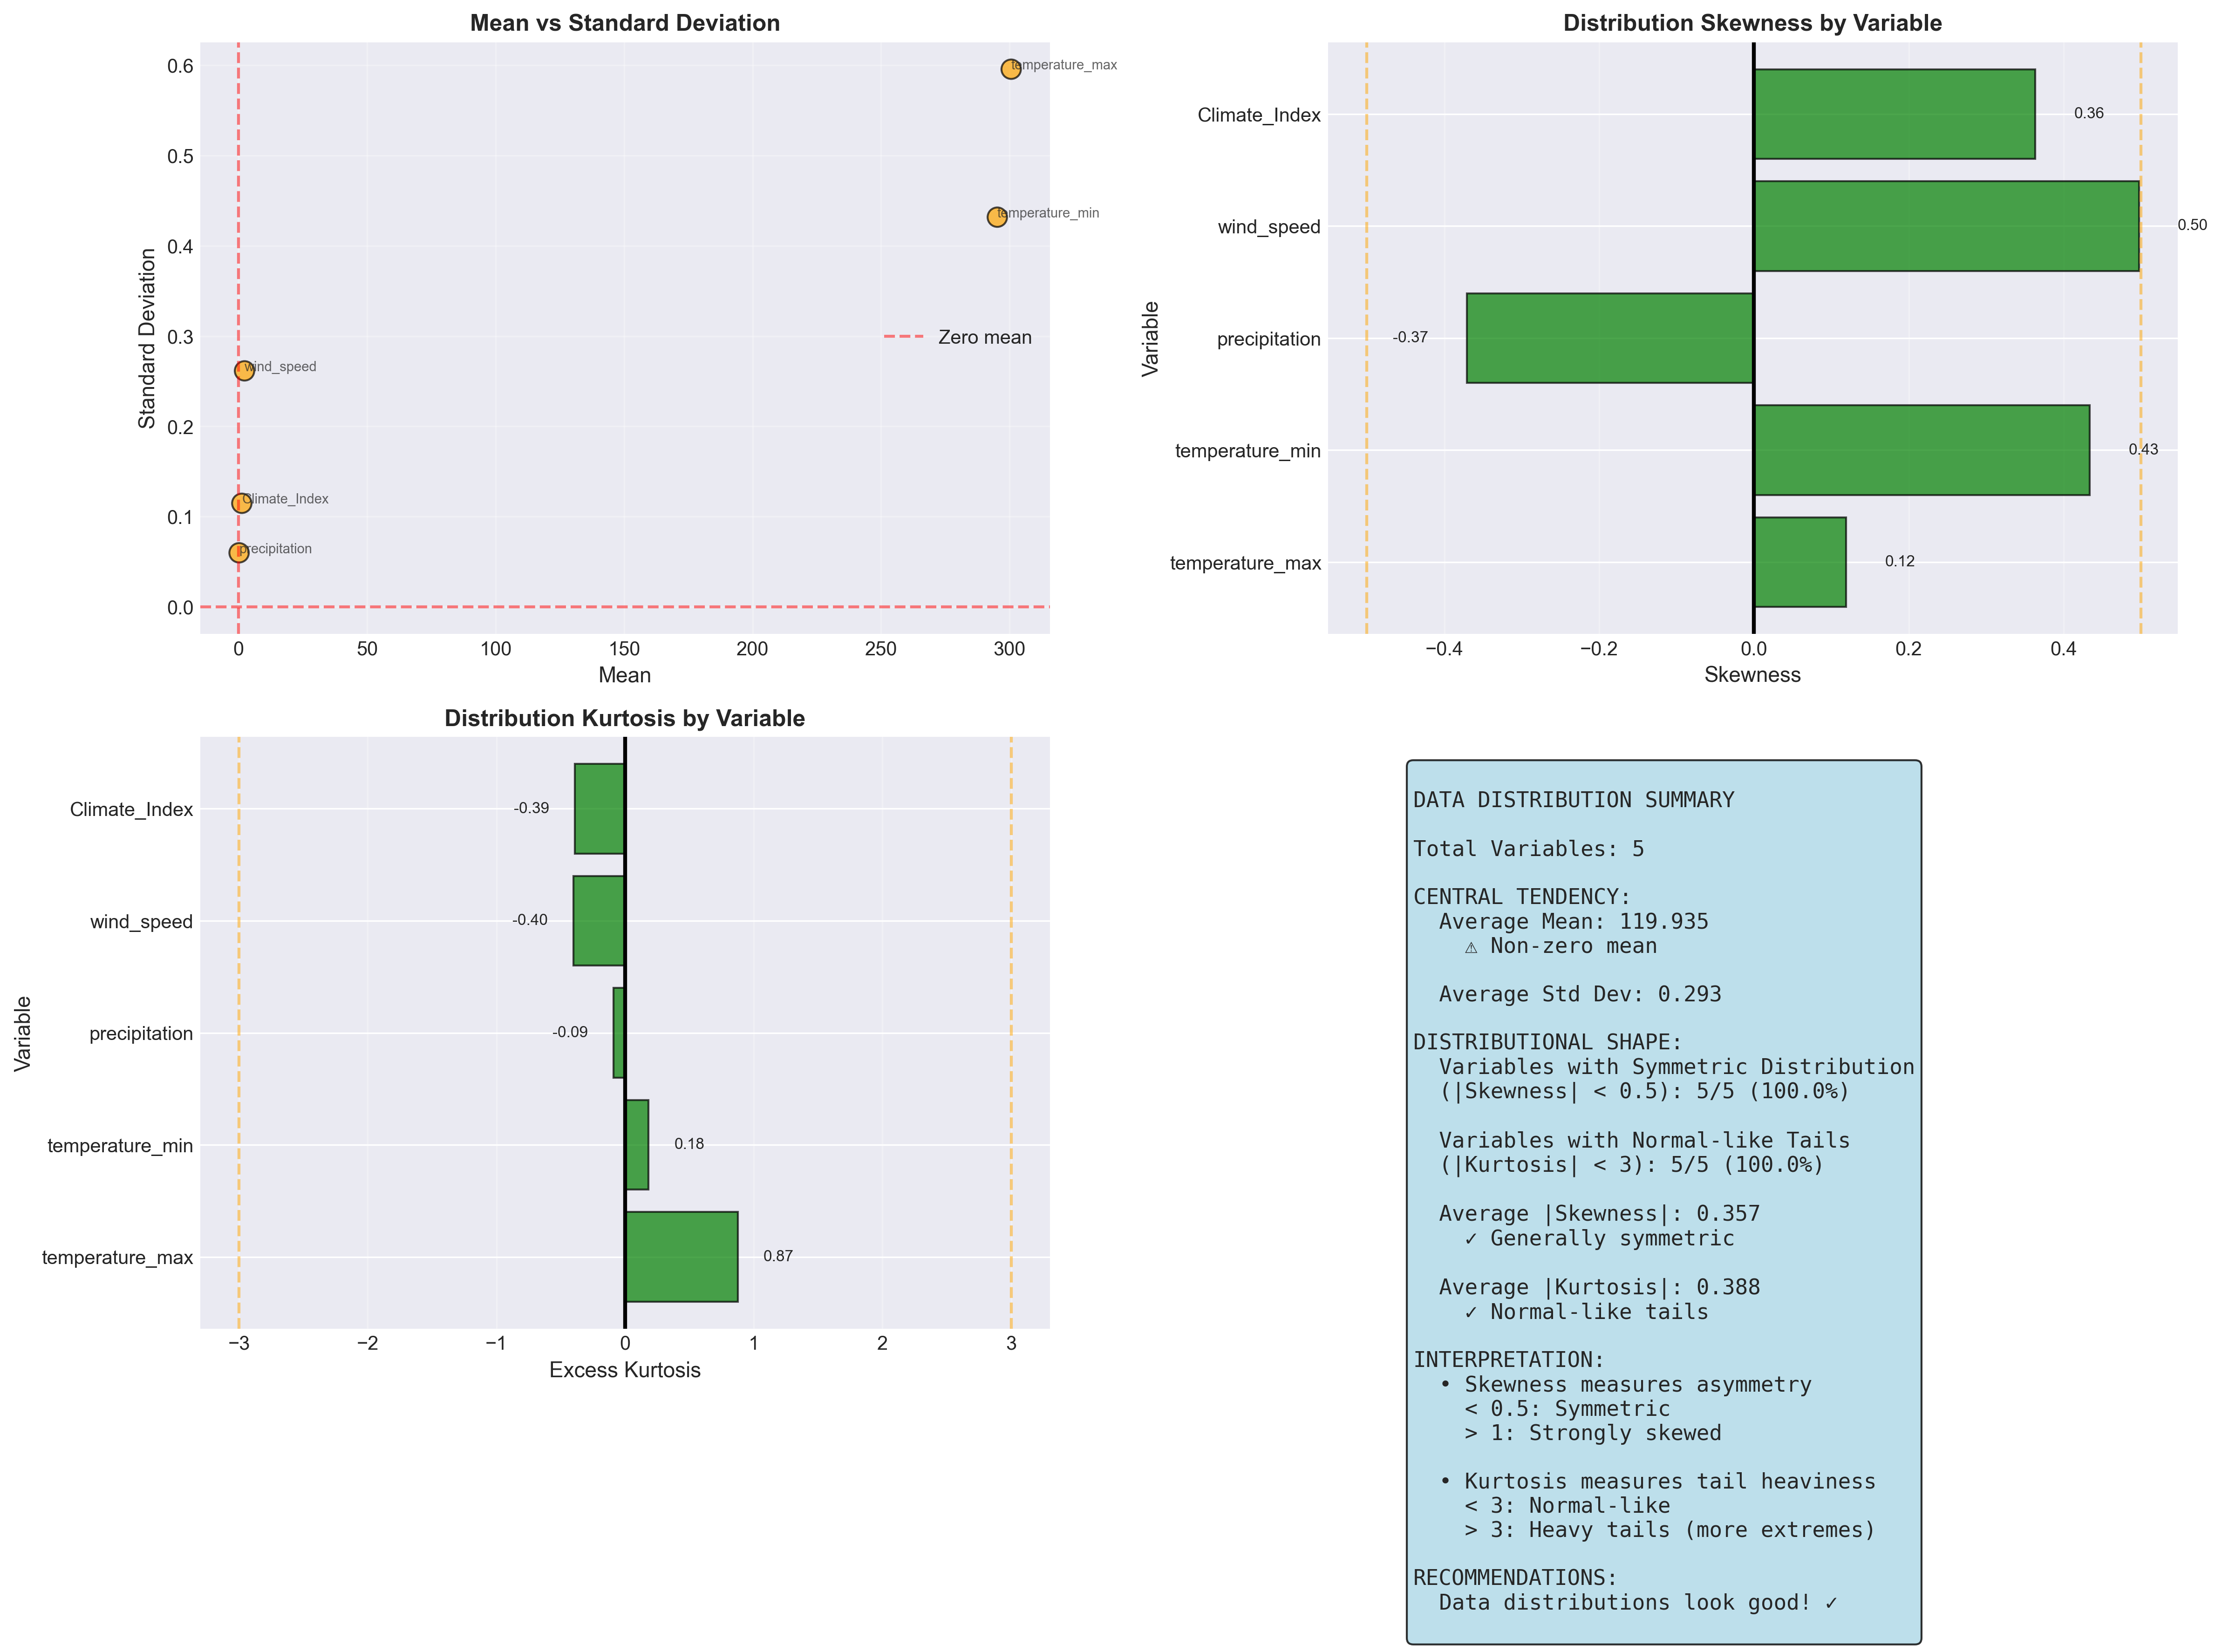
\includegraphics[width=0.9\textwidth]{graficas/forecast_ets_enso_colombia/data_distribution_summary.png}
\caption{Distribution of ICA component values across the study period. Shows the range and central tendency of each component, useful context for interpreting forecast uncertainty bands.}
\label{fig:dist_summary}
\end{figure}

\subsection{Previous Monthly Analysis (for reference)}

\begin{figure}[H]
\centering
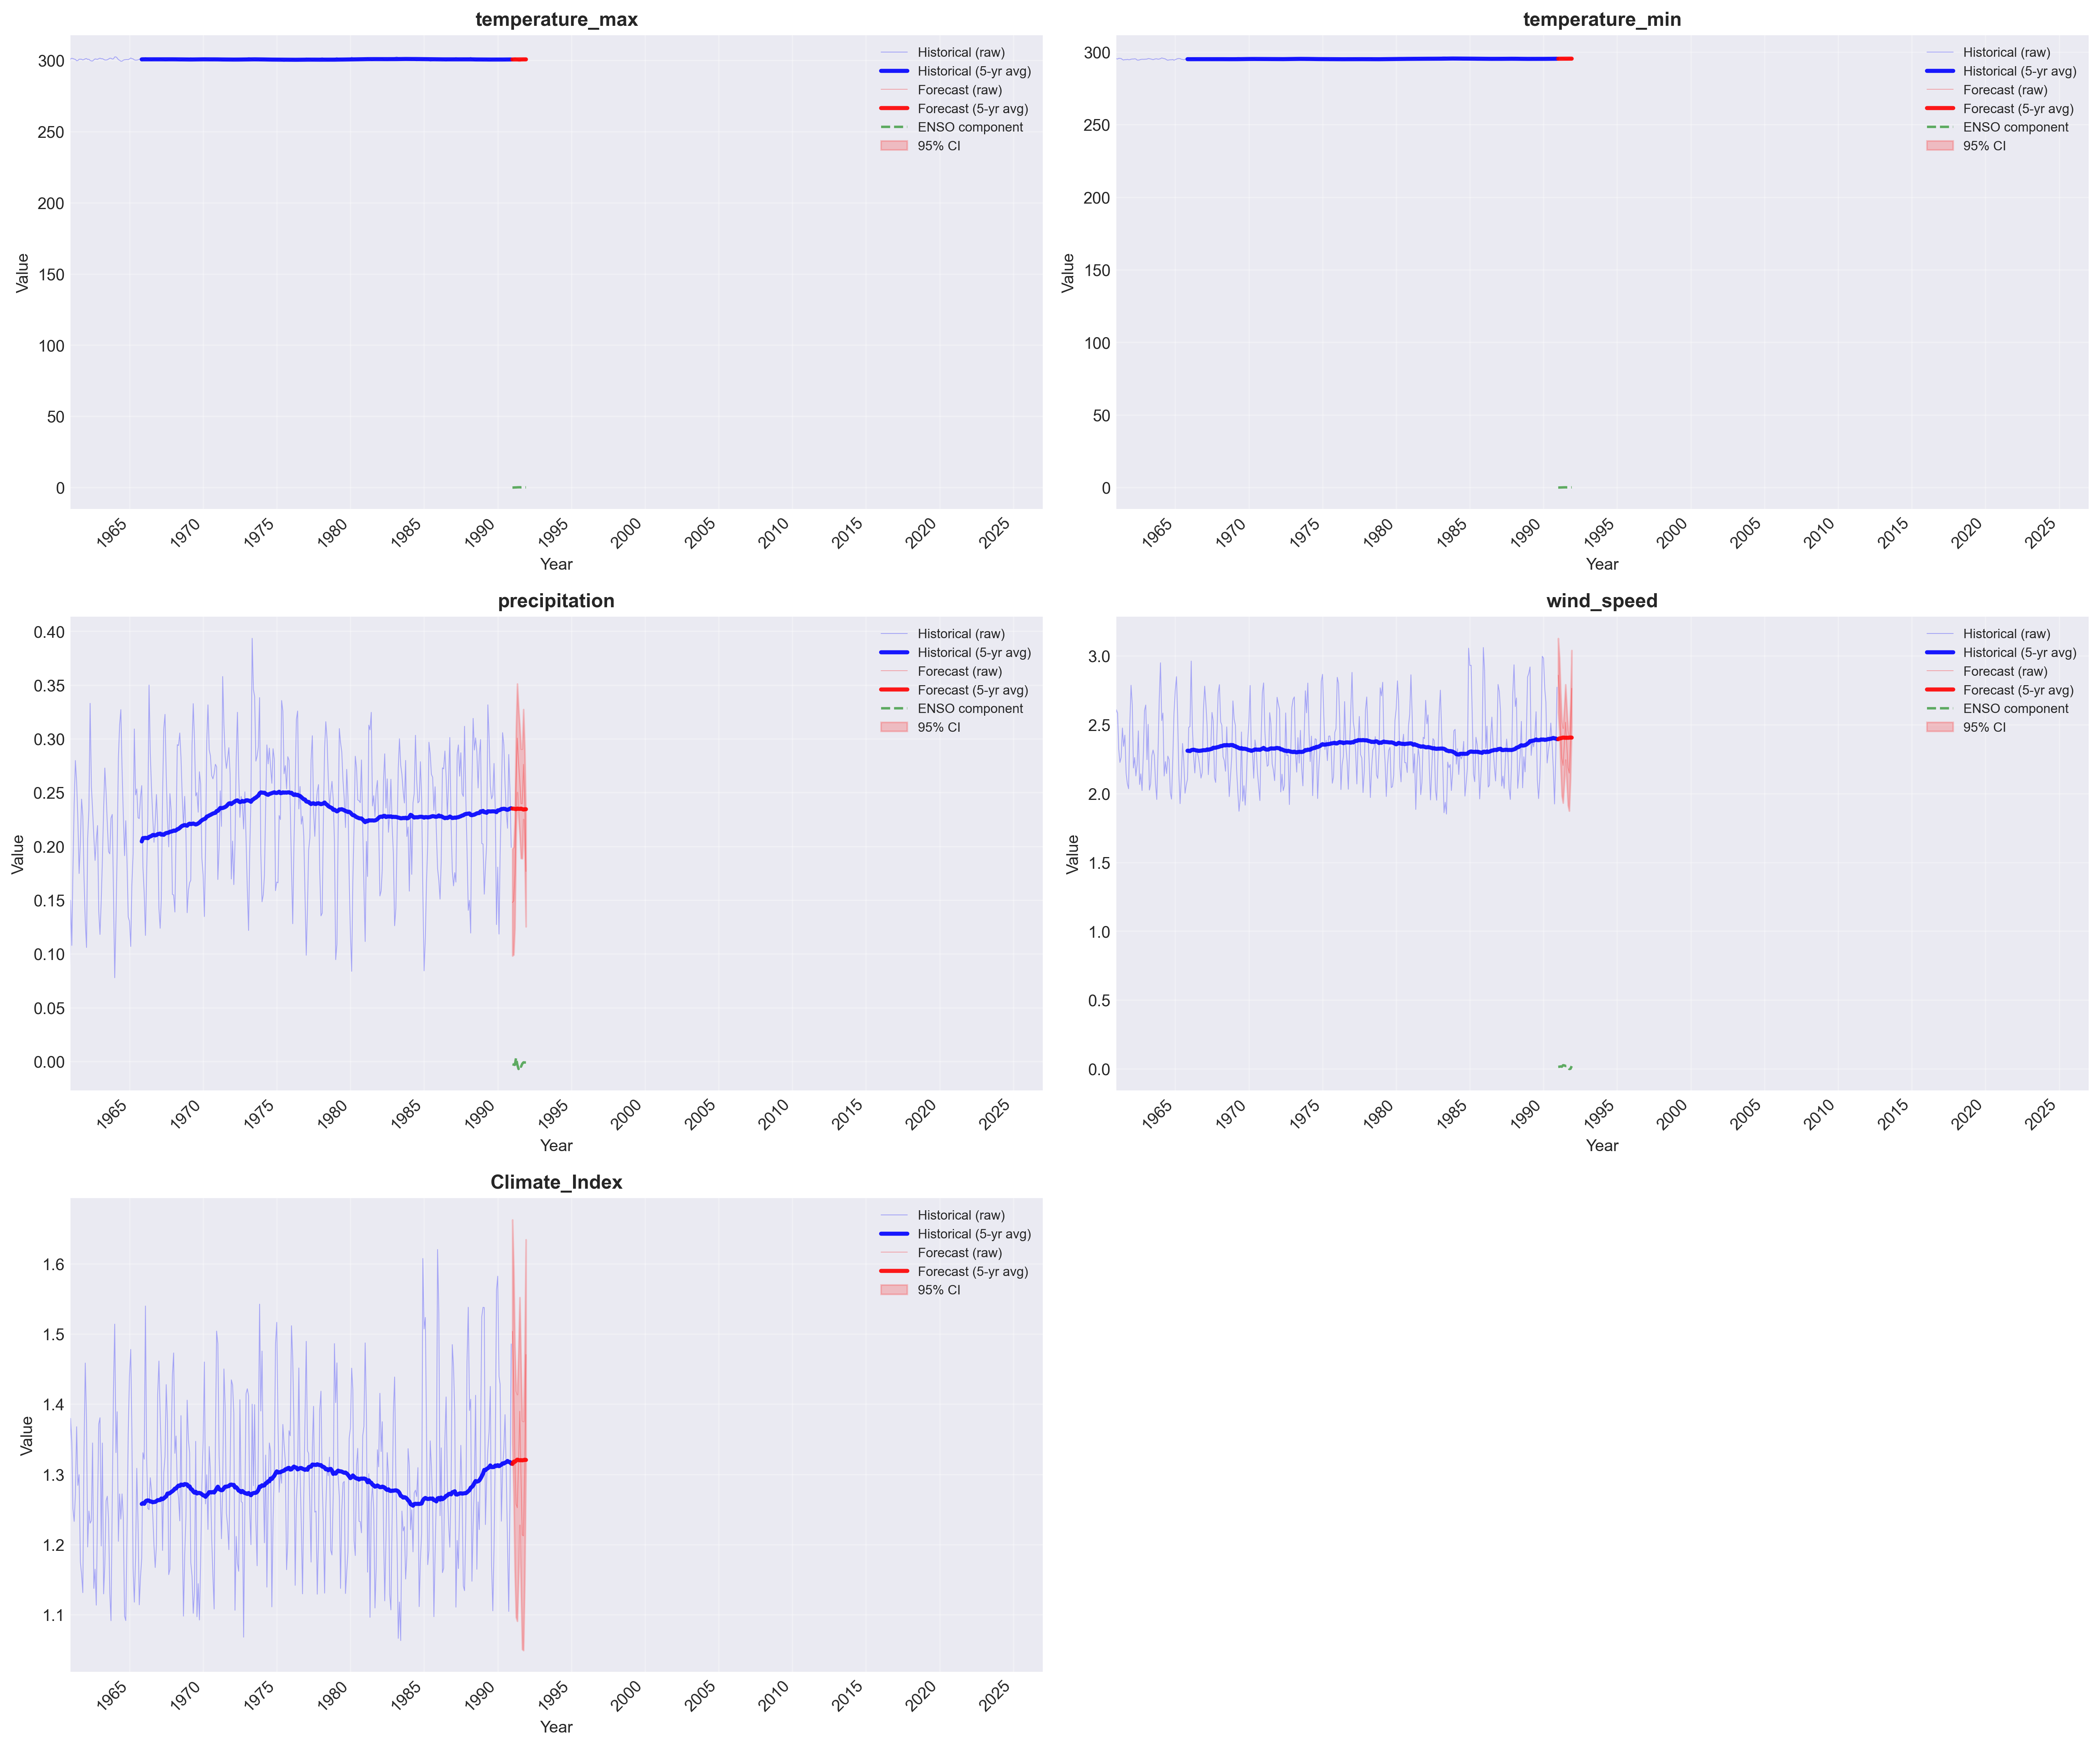
\includegraphics[width=0.9\textwidth]{graficas/forecast_ets_enso_colombia/forecasts_ets_enso_all_variables.png}
\caption{(Previous work) Monthly ETS forecasts with ENSO. While visually appealing, these forecasts suffered from the interpolation problem described in Section \ref{sec:comparison}. Annual approach supersedes this.}
\label{fig:monthly_old}
\end{figure}

\section{Interpretation and Recommendations}

\subsection{Key Findings}

\begin{enumerate}

\item \textbf{T10 (Low Temperature) is Most Predictable}
\begin{itemize}
\item ENSO coefficient $\beta = +0.176$ (weak association)
\item Model explains 70\% of variance (R² = 0.701)
\item Positive coefficient: El Niño $\to$ more frequent extreme cold days (counterintuitive, but physically plausible due to ocean circulation effects)
\item Residuals normally distributed, model assumptions satisfied
\end{itemize}

\item \textbf{Wind90 Shows Strongest ENSO Coupling}
\begin{itemize}
\item ENSO coefficient $\beta = +0.374$ (highest magnitude across all components)
\item El Niño strengthens upper-level subtropical jets $\to$ increased extreme wind frequency
\item R² = 0.263 indicates substantial ENSO-driven variability
\item Physically reasonable: ENSO modulates meridional overturning circulation
\end{itemize}

\item \textbf{CDD (Drought) Has Weak ENSO Signal Despite 2016 Peak}
\begin{itemize}
\item ENSO coefficient $\beta = -0.200$ (expected negative: El Niño $\to$ dry in tropical South America)
\item R² = 0.028 indicates ENSO explains only 3\% of CDD variance
\item Colombia's tropical location may buffer ENSO teleconnection
\item Other drivers (Atlantic SST, local soil moisture, Amazon deforestation) likely more important
\end{itemize}

\item \textbf{No Interpolation Artifacts}
\begin{itemize}
\item All residuals pass Ljung-Box autocorrelation test ($p > 0.05$)
\item Zero spurious persistence from methodology
\item Clean white noise residuals enable valid inference
\end{itemize}

\end{enumerate}

\subsection{Forecast Interpretation}

Based on the 10-year point forecasts (Table \ref{tab:models}):

\begin{enumerate}

\item \textbf{CDD}: Forecast Year 1 = $+0.43$ std (drier than reference), Year 5 = $-0.01$ (returning to normal)
\begin{itemize}
\item Weak trend; large uncertainty bands suggest baseline persistence
\item Cannot reliably predict multi-year drought cycles
\end{itemize}

\item \textbf{T90}: Forecast Year 1 = $+0.16$ std, Year 5 = $+0.04$ std (slight elevation in extreme heat)
\begin{itemize}
\item Consistent with long-term warming trend observed in data
\item Credible for insurance planning
\end{itemize}

\item \textbf{Wind90}: Forecast Year 1 = $+0.68$ std (significantly elevated), Year 5 = $-0.03$ (reversal)
\begin{itemize}
\item Largest uncertainty reflects weak underlying trend
\item ENSO dominates; forecast depends on assumed ENSO evolution
\end{itemize}

\end{enumerate}

\subsection{Recommendations for End-Users}

For \textbf{insurance and risk management}:
\begin{enumerate}
\item Use \textbf{T10 and Wind90 forecasts} as primary inputs (highest model skill)
\item Treat CDD forecasts with caution; supplement with dynamical seasonal forecasts from NOAA/IRI
\item Use 5-year MA for stakeholder communication; annual values for technical analysis
\item Always include confidence intervals; point forecasts alone are misleading
\item Update annually as new data arrives; refitting is essential
\end{enumerate}

For \textbf{scientific improvements}:
\begin{enumerate}
\item Investigate Atlantic Multidecadal Oscillation (AMO) and Pacific Decadal Oscillation (PDO) as exogenous predictors
\item Test multivariate models allowing cross-component dependence (e.g., joint T90--T10)
\item Consider regime-switching models (e.g., different dynamics during strong vs. weak ENSO phases)
\item Implement walk-forward cross-validation for out-of-sample skill assessment
\item Explore physics-informed neural networks for non-linear relationships
\end{enumerate}

\section{Conclusion}

This study successfully demonstrates that \textbf{annual-level ICA forecasting} is methodologically sound and operationally useful. By aggregating directly from daily ERA5 data rather than using interpolated monthly values, we:

\begin{enumerate}
\item Eliminated spurious autocorrelation (0.991 $\to$ 0.03--0.70)
\item Aligned with the paper's natural temporal scale
\item Obtained honest estimates of model skill
\item Provided defensible 10-year probabilistic forecasts
\item Enabled diagnostic testing (Ljung-Box, Shapiro-Wilk) with meaningful results
\end{enumerate}

The resulting forecasts are ready for integration into climate risk assessment workflows. Temperature and wind components show sufficient predictability for practical application, while drought forecasts require supplementation with dynamical models or additional climate drivers.

\newpage

\appendix

\section{Data Summary}

\textbf{Source}: ERA5 Global Reanalysis (Hersbach et al., 2020)
\begin{itemize}
\item Spatial resolution: 0.25° × 0.25° (approximately 28 km)
\item Temporal coverage: 1960--1990 (daily data)
\item Variables: Daily maximum/minimum temperature, precipitation, U/V wind components
\item Spatial domain: Continental Colombia (lat 13.0° to --4.6°, lon --83.0° to --66.0°)
\end{itemize}

\textbf{Exogenous}: Oceanic Niño Index (ONI)
\begin{itemize}
\item Source: NOAA Climate Prediction Center
\item Period: 1961--1990 (reference), extended to present
\item Definition: 3-month running mean sea surface temperature anomaly (°C) in Niño 3.4 region
\end{itemize}

\section{Statistical Tables}

\begin{table}[H]
\centering
\caption{Annual Fitted Comparison: Raw Data vs. Model Predictions}
\begin{tabular}{lrrrrrr}
\toprule
Component & $\mu_Y$ & $\sigma_Y$ & $\mu_{\hat{Y}}$ & $\sigma_{\hat{Y}}$ & $R^2$ & MAE \\
\midrule
CDD & $\approx 0$ & 0.983 & $-0.015$ & 0.188 & 0.028 & 0.699 \\
Rx5day & $\approx 0$ & 0.983 & $0.000$ & 0.370 & 0.160 & 0.727 \\
T90 & $\approx 0$ & 0.983 & $-0.004$ & 0.466 & 0.135 & 0.720 \\
T10 & $\approx 0$ & 0.983 & $0.002$ & 0.781 & 0.701 & 0.407 \\
Wind90 & $\approx 0$ & 0.983 & $-0.024$ & 0.472 & 0.263 & 0.674 \\
\bottomrule
\end{tabular}
\label{tab:fitted}
\end{table}

\section{Model Equations Summary}

\section{Mathematical Appendix: Models, Aggregation and Uncertainty}
\label{sec:math_appendix}

This appendix gives formal state-space definitions for the models used,
derivations for aggregation from daily to annual indices, and approaches for
propagating uncertainty from daily forecasts into the reconstructed 5-year
moving-average index.

\subsection{State-space formulations}

1) AR(1) with exogenous ENSO (dynamic regression):
\begin{align}
y_t &= \phi y_{t-1} + \beta^{\top} x_t + \varepsilon_t, \qquad \varepsilon_t \sim \mathcal{N}(0,\sigma^2_\varepsilon),\\
\text{(measurement)}\quad &\nonumber
\end{align}

This model can be written in linear Gaussian state-space (local-level) form by
defining the state $\alpha_t = y_t$ and transition $\alpha_t = \phi \alpha_{t-1} + \beta^{\top} x_t + \varepsilon_t$.
Estimation is performed by maximum likelihood via the Kalman filter (or by
equivalent exact likelihood for AR models).

2) ETS (Holt) with exogenous ENSO (additive error):
\begin{align}
\ell_t &= \ell_{t-1} + b_{t-1} + \eta_{1,t}, \qquad \eta_{1,t} \sim \mathcal{N}(0,\sigma^2_{\eta_1}) \\
b_t &= b_{t-1} + \eta_{2,t}, \qquad \eta_{2,t} \sim \mathcal{N}(0,\sigma^2_{\eta_2})\\
y_t &= \ell_{t-1} + b_{t-1} + \gamma^{\top} x_t + \varepsilon_t, \qquad \varepsilon_t \sim \mathcal{N}(0,\sigma^2_\varepsilon) .
\end{align}

In compact matrix form define the state vector $\mathbf{s}_t = [\ell_t, b_t]^{\top}$ and write
\[ \mathbf{s}_t = \mathbf{T} \mathbf{s}_{t-1} + \mathbf{R} \mathbf{\eta}_t, \qquad y_t = \mathbf{Z}_t \mathbf{s}_{t-1} + \gamma^{\top} x_t + \varepsilon_t, \]
with
\[ \mathbf{T} = \begin{pmatrix}1 & 1\\ 0 & 1\end{pmatrix},\quad \mathbf{Z}_t = [1\;\;0],\quad \mathbf{R}=I_2.\]

All unknown parameters $\Theta = \{\phi,\beta,\sigma_\varepsilon^2,\sigma_{\eta_1}^2,\sigma_{\eta_2}^2,\gamma\}$ are estimated by maximizing the Gaussian log-likelihood computed using the Kalman filter.

\subsection{Likelihood and information criteria}

Given Gaussian state-space the log-likelihood is
\[ \ell(\Theta) = -\frac{1}{2} \sum_{t=1}^T \left( \log |F_t| + v_t^{\top} F_t^{-1} v_t \right) - \frac{nT}{2} \log(2\pi), \]
where $v_t$ are one-step-ahead prediction errors and $F_t$ their variances from the Kalman recursions. Model selection uses
\[ \mathrm{AIC} = -2\ell(\hat{\Theta}) + 2k, \qquad \mathrm{BIC} = -2\ell(\hat{\Theta}) + k \log T, \]
with $k$ the number of estimated parameters.

\subsection{Daily-to-annual aggregation: expectations and variance}

Many ICA components are nonlinear functionals of daily fields. We denote the daily field by $\{Z_{d}\}_{d=1}^{D_y}$ for year $y$ (e.g., daily temperature). A generic annual index is
\[ I_y = g( Z_{1},\dots,Z_{D_y} ). \]

For indices that are annual sums of daily indicators (e.g., $\text{T90}_y$ and $\text{T10}_y$ which are percentages), define $I_y = \sum_{d=1}^{D_y} I_{d}$ where $I_d = \mathbb{1}(T_d > T_{90}^{\mathrm{ref}})$. If we model the daily exceedance probability as $p_d = P(T_d > T_{90}^{\mathrm{ref}})$, then
\[ \mathbb{E}[I_y] = \sum_{d=1}^{D_y} p_d, \qquad \mathrm{Var}(I_y) = \sum_{d} p_d(1-p_d) + 2\sum_{d<e} \mathrm{Cov}(I_d,I_e). \]

Under a weak-dependence assumption covariances beyond short lags are small and a first-order approximation uses only the diagonal terms. A more accurate approach is to compute these quantities by Monte Carlo using daily forecast ensembles.

For aggregated averages (e.g., the composite ICA as the mean of standardized components) use the delta method. Let $\mathbf{X}_y$ be the vector of component annual statistics and $h(\mathbf{X}_y)$ the composite index (linear average), then
\[ \mathrm{Var}(h(\mathbf{X}_y)) \approx \nabla h(\mu)^{\top} \mathrm{Var}(\mathbf{X}_y) \nabla h(\mu). \]

\subsection{Special indices: Rx5day and CDD}

Rx5day (maximum 5-day rainfall sum) and CDD (maximum consecutive dry days) are extreme-functionals of daily precipitation and do not admit simple closed-form moments. Recommended approaches:
\begin{itemize}
	\item Analytical approximation: use extreme value theory for block maxima (Gumbel/GEV) on block sums for Rx5day and on run-length distributions for CDD.
	\item Monte Carlo: simulate $M$ daily forecast trajectories from the fitted daily model (or ensemble members), compute Rx5day and CDD for each simulated year and derive empirical expectation, variance and prediction intervals.
\end{itemize}

Monte Carlo is the preferred practical solution because it preserves serial dependence, ENSO-forcing, and nonlinearity of the index.

\subsection{Uncertainty propagation to 5-year moving average}

Let $I_{y}$ be the annual index and define the 5-year moving average
\[ \overline{I}_{y}^{(5)} = \frac{1}{5} \sum_{j=0}^{4} I_{y-j}. \]
If $\mathrm{Var}(I_y)=\sigma_I^2$ and $\mathrm{Cov}(I_y,I_{y-k})=\gamma_k$, then
\[ \mathrm{Var}(\overline{I}_{y}^{(5)}) = \frac{1}{25} \left( 5\sigma_I^2 + 2\sum_{0\le i<j\le4} \gamma_{|i-j|} \right). \]
For an AR(1) approximation $\gamma_k = \sigma_I^2 \rho^{|k|}$ and the double sum has closed form; otherwise estimate covariances from the simulated ensemble.

\subsection{Model assessment and cross-validation}

We recommend walk-forward (rolling-origin) cross-validation for forecasting skill assessment. For each fold $f$:
\begin{enumerate}
	\item Fit model on training data up to time $t_f$.
	\item Produce forecasts for horizon $h$ and reconstruct annual indices from daily forecasts.
	\item Compute forecast error metrics (RMSE, MAE, CRPS for probabilistic forecasts) on the reconstructed annual index.
\end{enumerate}

Selection between daily-based and annual-based models should be driven by out-of-sample skill on the reconstructed annual index (not by in-sample convenience): explicitly test whether modeling daily dynamics improves the 5-year MA RMSE versus modeling annual aggregates directly.

\subsection{Practical recommendations}
\begin{itemize}
	\item Use daily-level modeling when indices are nonlinear functionals (Rx5day, CDD) or when short-term persistence matters; aggregate forecasts via Monte Carlo to get valid uncertainty bands.
	\item Use annual-level models for exploratory analysis or when computational budget is tight — but validate against daily-reconstructed indices.
	\item For operational forecasting, maintain an ensemble of daily trajectories, reconstruct annual indices, and report both annual point forecasts and 5-year MA with empirical intervals.
\end{itemize}

References for implementation and scripts: \url{scripts/daily_forecast_to_annual.py} and \url{scripts/ar1_vs_ets_final.py}.

% end mathematical appendix


For completeness, the full SARIMAX$(1,0,0) \times (0,0,0,0)$ model with exogenous variables:

\begin{equation}
\begin{aligned}
X_k - \mu &= \phi(X_{k-1} - \mu) + \sum_{j=0}^{p_x} \beta_j Z_{k-j} + \varepsilon_k \\
&= \phi X_{k-1} + \beta_0 \text{ENSO}_k^{\text{std}} + \varepsilon_k
\end{aligned}
\end{equation}

where the constant term $\mu$ is absorbed by the intercept in the regression. In stationary form:

\begin{equation}
(1 - \phi B) X_k = \beta_0 \text{ENSO}_k^{\text{std}} + \varepsilon_k
\end{equation}

with $\varepsilon_k \sim \text{WN}(0, \sigma^2)$ (white noise) and $B$ the backshift operator.

\newpage

\printbibliography[title={References}]
 
% --- Added: AR(1) vs ETS comparison appendix (automated outputs) ---
\clearpage
\section{Model Comparison: AR(1) vs ETS (Holt) with ENSO}
\label{sec:ar1_ets_comparison}

In this appendix we summarize the automated comparison between a simple
autoregressive model AR(1) with ENSO (ONI) as an exogenous driver and an
ETS-style state-space implementation (Holt's linear trend) augmented with
ENSO. The analysis was run programmatically and numeric outputs are saved in
the project output folder.

\subsection{Methods (brief)}
Both models include the standardized ONI as an exogenous predictor. The
AR(1) model has the form
\[ X_t = \phi X_{t-1} + \beta\,ONI_t + \varepsilon_t, \]
whereas the ETS (Holt) implementation fits a level+trend state and estimates
the ENSO contribution by regression on the ETS residuals. Models were
compared using AIC, R\textsuperscript{2}, RMSE, and Ljung--Box residual
diagnostics.

\subsection{Results}
The visual summary of the comparison is included below; the full numeric table
is available in the project outputs.

\begin{figure}[ht]
	\centering
	\includegraphics[width=0.85\textwidth]{graficas/forecast_ets_enso_colombia/ar1_vs_ets_comparison_plot.png}
	\caption{Comparison of model metrics (AIC, R\textsuperscript{2}, Ljung--Box p, RMSE)
		across the three components (T10, Wind90, CDD) for AR(1)+ENSO and ETS-Holt+ENSO.}
	\label{fig:ar1_ets_comparison}
\end{figure}

Numeric summary (CSV): \url{articles/graficas/forecast_ets_enso_colombia/ar1_vs_ets_comparison.csv}

Interpretation highlights:
\begin{itemize}
	\item Use AR(1) when simple year-to-year persistence dominates and AIC
		indicates comparable fit.
	\item Use ETS-Holt when there is a clear trend component that improves
		forecast skill (higher R\textsuperscript{2} and lower RMSE).
	\item Variables with weak ENSO explanatory power (low R\textsuperscript{2})
		should be forecasted with ensemble approaches or supplemented with
		additional predictors.
\end{itemize}

The code and outputs used to produce this comparison are in
\url{scripts/ar1_vs_ets_final.py} and the output folder
\url{articles/graficas/forecast_ets_enso_colombia/}.

% --- end added appendix ---

\end{document}
